\subsection{Vorgehen bei Entwicklung}
\subsubsection{Vorgehensmodell für transparentes ML}
Grundsätzlich ist es bei einem praktischen Problem der realen Welt empfohlen, dass bei der Entwicklung von Software mit Endnutzern und Domänenexperten zusammengearbeitet wird und der gemeinsame Prozess so gestaltet wird, dass Endnutzer und Domänenexperten Feedback geben können \cite{zhou20182d}. Hierfür haben \cite{zhou20182d} ein Modell entwickelt, welches \emph{twodimensional (2D) transparency space} heißt und in Abbildung \ref{Fig:2D-Transparenz} zu sehen ist. Dieses Modell beschreibt den Workflow des transparenten ML (vgl. Kapitel \ref{subsubsec_TML}) und integriert sowohl ML-Experten als auch Domänennutzer in den Entwicklungsprozess.
\begin{figure}[h]
    \centering
    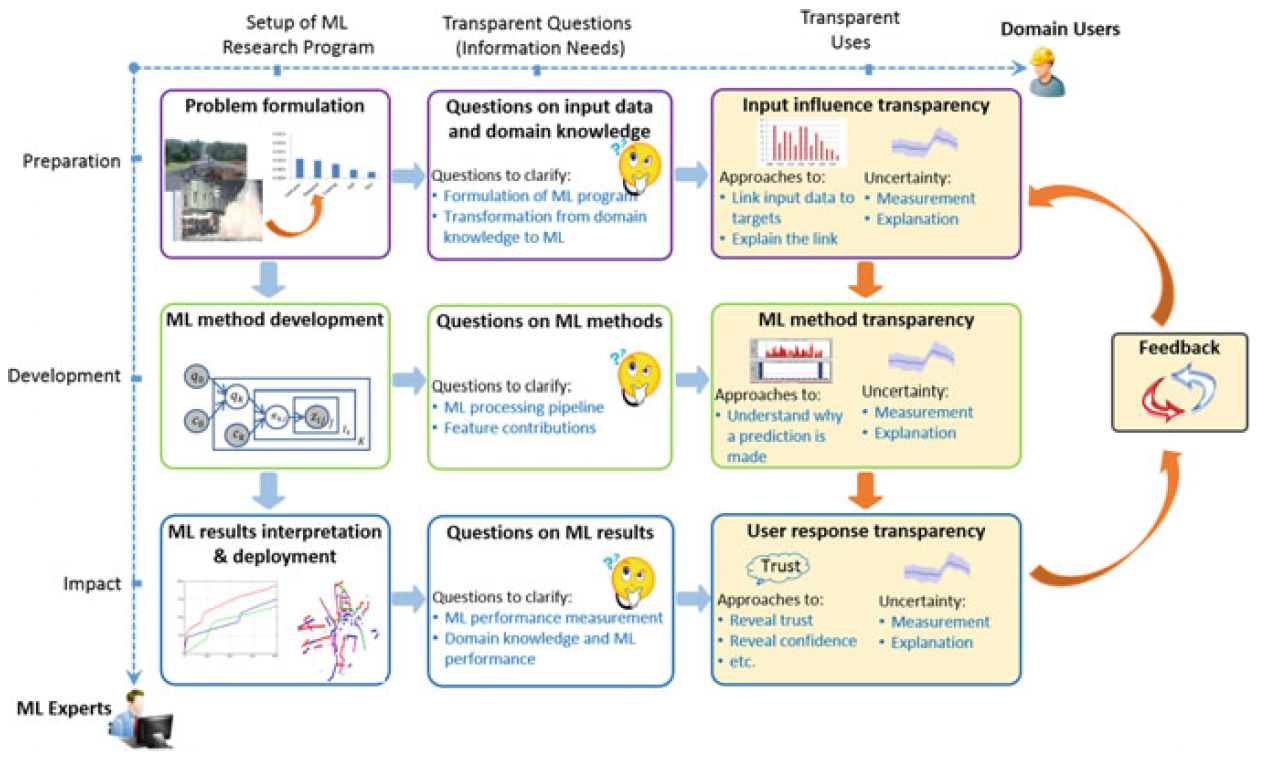
\includegraphics[scale=0.55]{pic/MA-Bilder/Literaturrecherche/4-2D-TransparencyWorkflow.PNG}
    \caption{2D transparency space, entnommen aus \cite{zhou20182d}}
    \label{Fig:2D-Transparenz}
\end{figure}

Aus Nutzerperspektive ergeben sich nach diesem Vorgehen drei Hauptaspekte. Zunächst wird das ML-Forschungsprogramm eingerichtet, was der Problemdefinition dient \cite{zhou20182d}. Gleichzeitig sollten Nutzer sogenannte \emph{transparente Fragen} stellen. Hier werden Informationsbedarfe für das ML-System aufgedeckt und beantwortet. Während der Vorbereitung ist beispielsweise wichtig, wie das Problem in ML überführt wird. In der Entwicklungsphase hingegen kann interessant sein, wie auf Daten zugegriffen wird. Wie die Leistung oder die Interpretation der Ergebnisse aussieht, sind transparente Fragen, welche während des Deployments stattfinden. Der dritte Baustein aus Nutzerperspektive ist der \emph{transparente Nutzen}. Während der Vorbereitung sollte verständlich gemacht werden, in welcher Form sich Inputs auf Outputs auswirken. Gleichzeitig sollen Unklarheiten über die Geschäftsanforderungen an das ML-System aufgelöst werden. Weiter sollte die ML-Methode selbst transparent gemacht werden, indem dessen Funktionsweise dargelegt wird. Eine Frage, welche hier beantwortet werden sollte ist z.B. \enquote{Warum wird diese mithilfe von Wissen über die Domäne Entscheidung getroffen?}. Während des Deployments sollten Reaktionen der Benutzer untersucht werden, um deren Vertrauen und Zuversicht zum ML-System zu stärken \cite{zhou20182d}. Ein wichtiger Bestandteil sind die Feedback-Schleifen. Sollte zum Ende des Projektes herausgefunden werden, dass Nutzer kein Vertrauen in das System haben, sollte die Problemdefinition und die Art der Überführung des Domänenproblems in ein ML-System erneut überdacht werden \cite{zhou20182d}.

Auch \cite{vaughan2020human} weist darauf hin, wie wichtig es ist verschiedene Stakeholder einzubeziehen, um dessen Bedürfnisse zu kennen. Dies sei besonders wichtig, um den Einsatz des ML-Systems im realen Kontext einschätzen zu können. Mögliche Stakeholder sind: Entwickler, Designer, Data Scientists, Manager, Regulierungsbehörden, Nutzer, Personen, welche in sonstiger Weise vom System betroffen sind.

Stakeholder früh einzubinden kann weiter das Problem des kognitiven Bias' bei Nutzern lösen, welcher bewirkt dass sie Erklärungen falsch oder anders verstehen. Erklärungen sollten Nutzern früh präsentiert werden, auch wenn dies bedeutet, dass noch Fehler in den Erklärungen vorhanden sein könnten\cite{nourani2021anchoring}. Für das Präsentieren der Erklärungen empfehlen \cite{nourani2021anchoring} zu Beginn high-level-Erklärungen, um ein grundsätzliches Bild darüber zu schaffen, wie das System funktioniert. Danach sollten einzelne Instanzen gezeigt werden. Die Erklärmethode sollte hier bewusst gewählt werden.

%\cite{hoang2021aid} haben AID: Active Distillation Machine to Leverage Pre-Trained Black-Box Models in Private Data Settings: aus bestehenden System Transparenz über Vorhersagen gewinnen, ohne auf alle Daten zugreifen zu dürfen --> Sicherstellung von Privacy. Dies wird durch die folgenden Module ermöglicht. Ausgehend von einem Blackbox-Modell, das auf privaten EHR -Daten trainiert wurde, lernt AID (I) ein Surrogatmodell, das globale und lokale interpretierbare Repräsentationen enthält; und (II) wendet eine aktive Strategie an, um das Blackbox-Modell sequentiell nach markierten Daten abzufragen, um sein Wissen in diese Repräsentationen zu destillieren.

%\cite{hernandez2021explainable} EU Proposal for Artificial Intelligence Act, 2021 sagt hochrisikosysteme (z.B. Luftfahrt, was Thema des Papers ist) sollen folgendes erfüllen: 1. Verwendung hochwertiger Trainings-, Validierungs- und Testdaten 2. Verwendung von Dokumentations- und Entwurfsprotokollierungsfunktionen, die eine kontinuierliche Dokumentation gewährleisten 3. Gewährleistung von Transparenz und Information der Nutzer über die Anwendung von KI-Systemen 4. Sicherstellung der menschlichen Aufsicht während des gesamten Prozesses 5. Sicherstellung der Genauigkeit, Robustheit und Cybersicherheit des Systems

\subsubsection{Transparenz während der Implementation}
Auch während der Implementation gibt es Maßnahmen, welche das ML-System transparenter machen. So empfiehlt z.B. \cite{huvc2021anomaly} das Anwenden einfacher Methoden.
Unterstützt werden kann transparente Entwicklung durch eine Toolbox namens Bob \footnote{https://www.idiap.ch/software/bob/}. Diese Toolbox bietet (Python-/C++)-Entwicklern Hilfestellungen bei der Siganlverarbeitung und dem ML. Unterstützt wird Reproduzierbarkeit durch Protokolle, aber auch durchschaubarer Code, Dokumentationen und Unit-Tests. 

Den Ansatz der Vereinfachung verfolgen auch \cite{zucker2020arbiter}, die eine eigene domänenspezifischen Sprache entwickelt haben, welche im Rahmen des ethischen ML neben Fairness, Zurechenbarkeit und Reproduzierbarkeit auch Transparenz gewährleistet. Unter einer domänenspezifischen Sprache, werden Programmiersprachen verstanden, welche nur in einem bestimmten Kontext eingesetzt werden. Hierdurch sind sie jedoch auch etwas begrenzter in ihrer Funktionalität. Diese domänenspezifische Sprache heißt \emph{Arbiter} und ist außerdem deklarativ. Dies bedeutet, dass Nutzer angeben, welches Ziel zu erreichen ist und das System selbst bestimmen kann, wie dies zu erreichen ist \cite{van2004concepts}. Transparenz während der Entwicklung wird mithilfe von \emph{Arbiter} vor allem dadurch geschaffen, dass Python Code kürzer dargestellt wird. Außerdem wird klarer herausgestellt, was eine bestimmte Zeile Code tut. Ein Beispiel für die Nutzung von \emph{Arbiter} ist in Abbildung \ref{Fig:Arbiter} zu sehen.
\begin{figure}
    \centering
    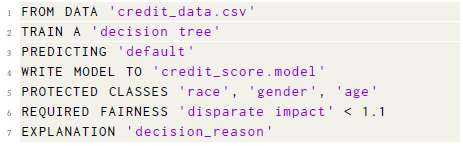
\includegraphics[scale=0.8]{pic/MA-Bilder/Literaturrecherche/45-CodeSnippet.PNG}
    \caption{Beispiel Arbiter, entnommen aus \cite{zucker2020arbiter}}
    \label{Fig:Arbiter}
\end{figure}

\subsubsection{AutoML}
Bei der Entwicklung eines ML-Systems kann es vorkommen, dass unterschiedliche Algorithmen ausprobiert werden. Zur automatisierten Unterstützung kann hierfür AutoML Anwendung finden. Dies sind Methoden, welche die Algorithmenauswahl und die Abstimmung der Parameter übernehmen, da es für Menschen zu aufwendig sein kann, dies händisch für eine Vielzahl an Möglichkeiten durchzuprobieren \cite{wang2019atmseer}. Um diesen automatischen Prozess transparent zu machen haben \cite{wang2019atmseer} das Tool \emph{ATMSeer} entwickelt. Dies ist ein Visualisierungstool, welches es Entwicklern ermöglicht einen Überblick über den AutoML-Prozess zu bekommen oder Statistiken auf unterschiedlichen Granularitätsebenen anzeigen zu lassen. 
%AuotML auch empfohlen von: \cite{waring2020automated}

\subsubsection{Verteiltes Lernen}
\begin{figure}[h]
    \centering
    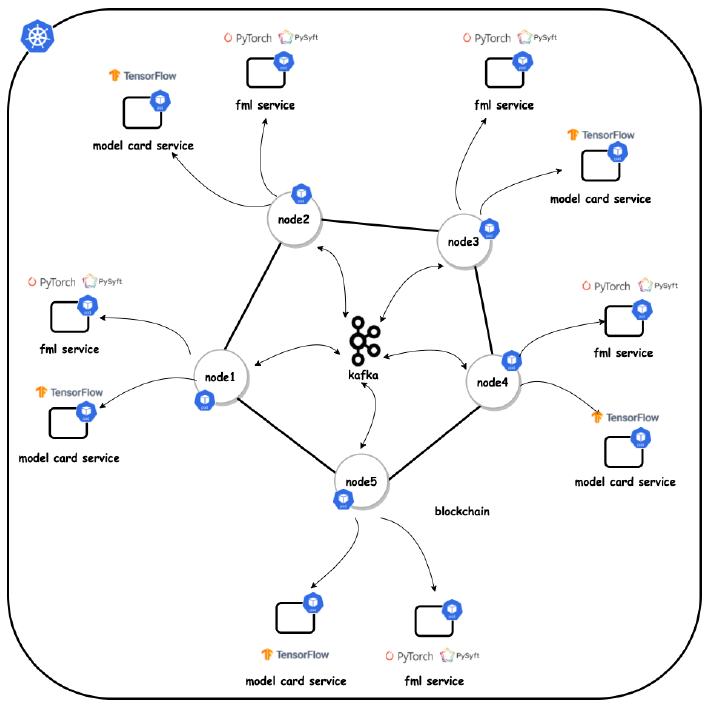
\includegraphics[scale=0.45]{pic/MA-Bilder/Literaturrecherche/56-BassaMLArchitektur.PNG}
    \caption{Architektur von Bassa-ML, entnommen aus: \cite{bandara2022bassa}}
    \label{Fig:Bass-ML-Architektur}
\end{figure}
Eine weitere Besonderheit bei dem Trainieren von ML-Modellen während der Entwicklung ist das verteilte Lernen. Dies sollte ursprünglich Datenschutzprobleme lösen, jedoch arbeiten die meisten Ansätze in der Praxis mit zentralisierten Koordination, welche anfällig für Angriffe von außen sind. Weiter besteht ein Problem beim verteilten Lernen darin, dass nicht klar ist, woher welche Daten stammen \cite{bandara2022bassa}.
\cite{bandara2022bassa} haben eine transparenzschaffende Maßnahme mithilfe der Blockchain-Technologie implementiert, welche Vertrauen und Transaprenz über die im verteilten Lernen erstellten Modelle schaffen soll. Ihre Lösung heißt Bassa-ML, welche ModelCards in einer Blockchain speichert und die Historie der verschiedenen Modelle transparent macht. Jeder Teilnehmer des Netzwerkes erstellt lokale Modelle und die zugehörigen ModelCards, welche zu lokalen Modellen aggregiert werden können, wenn Blöcke für das Block-Chain-Netzwerk erstellt werden. Die grobe Systemarchitektur ist schematisch in Abbildung \ref{Fig:Bass-ML-Architektur} dargestellt.

Auch \cite{zerka2020blockchain} machen sich die Vorteile von Block-Chain-Ansätzen zu nutze. Sie entwickelten \emph{Chained Distributed Machine learning (C-DistriM)}. Vorteile von solchen Ansätzen bestehen vor allem in der Transparenz über die Herkunft der Daten und in der Überwachung des Lernprozesses \cite{zerka2020blockchain}.